\chapter{Implementation Design}\label{ch:implementation}
Given the context and background surrounding the IEEE 2030.5 Protocol, we can begin examining the considerations taken when designing our implementation.

\section{Programming Language}
The operating context of IEEE 2030.5 greatly influences the software development tools that are suitable for implementation.
When choosing a programming language, we must consider:

\begin{itemize}
    \item \textbf{Device resource constraints} - Many existing IEEE 2030.5 compliant devices are constrained by the clockspeed of the onboard CPU, and the amount of onboard memory.
    For example, the "Gen5 Riva" smart meter by Itron, possesses a 600Mhz processor, and 256Mb of RAM.\cite[]{Gen5Riva}
    \hfill \break
    Therefore, we desire a programming language with minimal runtime overhead, and low-cost abstractions.
    \item \textbf{Cross-platform capabilities} - Given that our client may be deployed on embedded hardware, writing code in a language that can be compiled to a wider range of CPU and hardware configurations is desirable. 
    For this reason, we saw EPRI choose to implement their client in the C programming language.
    \item \textbf{Security} - In 2019, Microsoft attributed 70\% of all CVEs in software to be caused by memory safety issues, in the last 12 years. \cite[]{SecurityMemorySafety}
    As we've previously established improving the security of end user energy devices is part of the core rationale behind IEEE 2030.5. For that reason, developing our client in a language that is memory safe would work towards this goal.
    \item \textbf{Concurrent programming support} - By nature of the protocol, an IEEE 2030.5 client is an I/O bound application. For that reason, we desire a programming language that provides us with abstractions for event-driven architecture, such that operations can be performed while waiting on I/O, even on a single threaded device.
\end{itemize}


\subsection{Rust}
The Rust programming language is a high-level, general purpose programming language that has been strongly influenced by the successes of other programming languages, both industrial and academic
Rust will be used to develop our IEEE 2030.5 client implementation as it addresses all the aforementioned considerations.

\begin{itemize}
    \item Rust provides us with high-level abstractions, but with a focus on performance, and only 'paying' (in terms of available computer resources) for what you use. For that reason, Rust has seen usage in both application and systems level programming.
    \item Although Rust is by no means a universal programming language like C, it has a growing presence in embedded development, and as such has a reasonable degree of portability.
    \item While writing a variation of Rust called 'safe' Rust, the programming language is, outside of compiler bugs, completely memory safe, without the runtime overhead of a garbage collector. When writing 'unsafe' rust, raw pointers may be dereferenced, where by the compiler is no longer able to guarantee memory safety. For that reason, our implementation will be done using purely safe Rust.
    \item Through it's type system, Rust also eliminates the possibility of a data race when working with multiple threads of execution. Furthermore, Rust has native support for asynchronous programming, with concurrency-runtime-independent await and async syntax.
\end{itemize}

Rust's high-level abstractions furthermore lend themselves to the imposed reliability of the client, in that all expected errors are to be handled at compile-time. The Rust algebraic sum types 'Option' and 'Result' enable programmers to handle errors, in order to use the output of a process.
This is contrasted to a language like C++, where runtime exceptions are used to denote errors in the standard library, of which the language does not force the programmer to handle at compile-time.

\section{Operating System}
Despite the desire to write code that is portable, we will nonetheless require operating-system-specific functionality, and as such will need to target a single operating system. Then, we can provide an interface for device manufacturers to swap out should they want to use the client on a different operating system.

Of great consideration when choosing an operating system is the aforementioned 'Aggregator' model for IEEE 2030.5, where by our client would be deployed on a dedicated server, or in the cloud. In this circumstance, it's very much likely an operating system running on the Linux kernel is to be used, due to it's prevalence in server operating-systems.
Whilst there exist purpose built IOT-device operating systems, they are built and optimised for low-spec low-power usage devices, and as such would not be appropriate at scale such as under this model.

Furthermore, there exist very lightweight Linux based operating systems for low-spec devices, making Linux the best choice for our targeted operating system.

\section{Common Library}
As discussed, the IEEE 2030.5 specification makes no distinction between clients \& servers, aside from the fact that servers expose resources, and clients interact with resources. 
For that reason, our client implementation will also produce a common library, that would be used one by developing a IEEE 2030.5 server implementation in Rust.

In this context, it's reasonable to draw inspiration from the EPRI implementation of an IEEE 2030.5 client, and define a series of interfaces that make use of OS specific APIs, such that a device manufacturer need only re-implement those interfaces when porting our software to a different OS.

\subsection{Resource Data Types}
The most important, and largest part of this common library is the internal representation of resources, the data communicated between client \& server. These resources are described precisely in an XSD.
Resources range from data that may be used by the electric utility, such as the current load of the device, to resource metadata, such as the rate at which a client should poll a server for a given resource, or what URI endpoint can be used to access a given resource, in the case of a Link resource.
In both specification and schema, these data structures are separated into packages, and sub-packages. 

Whilst the 2030.5 specification makes no mention of the object oriented programming paradigm, OOP inheritance underpins the design of all resources, including both multi-level and hierarchial inheritance.
As such, for the purpose of code reuse, many base types appear in the 'common' package; data structures extended by many others.

\subsubsection{Representing Resources in Rust}
Rust, despite being influenced by OOP, does not posses the notion of a class, like in languages like C++ or Java, and as such does not define shared behaviour of types through inheritance from a common parent type. 
Rather, Rust defines shared behaviour through traits, where shared behaviour refers solely to the methods that we can call on that type, as per the traits a type implements.
In this sense, Rust does not concern itself with what a type is or what that type stores, it concerns itself only with the traits a type possesses.

Traits themselves do support inheritance. One can have traits that require other traits to be implemented for a given type. However, this does not change the fact that traits only represent behaviour. 
There is no way to have a data structure inherit the internal members of another.

\begin{figure}[H]
    \begin{center}
        \begin{lstlisting}
            pub trait Resource {
                fn get_href(&self) -> Option<&str>;
            }
        \end{lstlisting}
        \caption{A Rust trait representing the IEEE 2030.5 "Resource" data type}
    \end{center}
\end{figure}



\begin{figure}[H]
    \begin{center}
        \begin{lstlisting}
            pub trait List : Resource {
                fn all(&self) -> UInt32;
                fn results(&self) -> UInt32;
            }
        \end{lstlisting}
        \caption{A Rust trait representing the IEEE 2030.5 \texttt{List} data type}
    \end{center}
\end{figure}

In Figure 5.2, we have a Rust trait that describes the behaviour of the List base type. All lists are resources, and thus we have a trait restriction that all types implementing List must first implement the Resource trait.

This is the extent of native inheritance in rust. We can specify the exact behaviour of types that belong to a trait in detail, but we cannot influence how that behaviour is achieved.

\subsubsection{Emulating inheritance in Rust}

As a result, we're forced to emulate the inheritance of data structure members in Rust, of which there are two approaches:

\begin{itemize}
    \item Composite an instance of the base type into type definitions 
    \item Repeat all inherited members in type definitions
\end{itemize}

Regardless of the approach, we still do not have have polymorphism using the base-types of resources.
To allow for polymorphism a trait must be defined for each base-type, and then those trait functions need be implemented for every type that extends the base type. 
This is unavoidable duplicate code, not ignoring the possibility of generating said code.
The extent to which polymorphism is required in the final client implementation is yet to be determined. In this case, we can refer to the EPRI client implementation, 
where they provide device manufacturers an interface for handling resources using polymorphism.
Thus, when determining how we will emulate inheritance, we let the ease at which polymorphism can be allowed influence our decision


\subsubsection{Inheritance via Composition}

If we were to implement the first of the two approaches, we can make use of an existing Rust library to reduce the amount of boilerplate required to implement polymorphism.
This library operates on the basis that inheritance can be replicated via composition. If a data type were to contain a member that implements a given trait, there is no reason for that outer struct to not be able to implement that trait by simply calling upon the underlying member.


\begin{figure}[H]
    \begin{center}
        \begin{lstlisting}
            #[inheritable]
            pub trait Resource {
                fn get_href(&self) -> Option<&str>;
            }

            pub struct ResourceObj {
                href: Option<String>
            }

            impl Resource for ResourceObj {
                fn href(&self) -> Option<&str> {
                    self.href.as_str()
                }
            }
        \end{lstlisting}
        \label{fig:resinher}
        \caption{Rust code required to represent the IEEE 2030.5 "Resource" data type using 'inheritance-rs'}
    \end{center}
\end{figure}

\begin{figure}[H]
    \begin{center}
        \begin{lstlisting}
            #[derive(Inheritance)]
            pub struct List {
                #[inherits(Resource)]
                res: ResourceObj,
                all: UInt32,
                results: UInt32,
            }
        \end{lstlisting}
        \label{fig:listinher}
        \caption{A Rust data type representing an IEEE 2030.5 \texttt{List} using 'inheritance-rs'}
    \end{center}
\end{figure}


Figures 5.3 and 5.4 show how this library, 'inheritance-rs' \cite[]{inheritancers} is used to reduce the boilerplate necessary to inherit data members. 
In Figure 5.3, we mark the Resource trait as 'inheritable' and then implement that trait on a type that holds the necessary members, our bare minimum 'base' type. 
In Figure 5.3, we compose an instance of that base type into a type that would normally inherit from it. Then, we tell the library to generate the code, at compile-time, that would allow List to implement the Resource trait.
This generated code simply calls the underlying ResourceObj member when the href function would be called on a list.

The major flaw in this approach is that for every single type that is used as a base type, a trait, and a base implementation of that trait needs to be written.
Given that there are just under 700 data types in the IEEE 2030.5 specification schema, we must consider alternatives.


\subsubsection{XSD to Rust types}

If we were to implement the second approach, an existing Rust library can be used to automate the process of defining data types altogether.
This of course draws on the fact that the IEEE 2030.5 XSD is entirely self-contained, and follows XSD guidelines by W3C. As such, generating rust data types from it is a reasonable approach.
One such way to automate this process would be to design and implement our own XSD parser, however, we are not the first to require this tool. 

On the Rust public crates registry there are several XSD parsers, many of which existing to solve very similar problems; implementing standardised communication protocols in Rust.
However, for that reason, many of these implementations are developed until they meet the creators needs, at which point the tool is no longer maintained.

Of the most complete parsers, one particular implementation stands out. This particular implementation supports hierarchial inheritance and makes reasonable assumptions on the internal representations of primitive data types.
\texttt{xsd-parser-rs} by \texttt{Lumeo}, was created for use in their \texttt{Open Network Video Interface Forum Client}, software with requirements not dissimilar from that of IEEE 2030.5.

\begin{figure}[H]
    \begin{center}
        \begin{lstlisting}
            #[derive(Default, PartialEq, Debug, YaSerialize, YaDeserialize)]
            #[yaserde(namespace = "urn:ieee:std:2030.5:ns")]
            pub struct List {
                // The number specifying "all" of the items in the list. 
                // Required on a response to a GET, ignored otherwise.
                #[yaserde(attribute, rename = "all")]
                pub all: Uint32,
            
                // Indicates the number of items in this page of results.
                #[yaserde(attribute, rename = "results")]
                pub results: Uint32,
            
                // A reference to the resource address (URI). 
                // Required in a response to a GET, ignored otherwise.
                #[yaserde(attribute, rename = "href")]
                pub href: Option<String>,
            }
        \end{lstlisting}
        \label{fig:listauto}
        \caption{A Rust data type representing an IEEE 2030.5 \texttt{List} as generated by \texttt{xsd-parser-rs}}
    \end{center}
\end{figure}

Figure 5.5 is what \texttt{xsd-parser-rs} currently produces for the List resource. In this figure, it's parsed that the List type inherits from the Resource type, and included the href data member accordingly. It's also included the documentation as found in the schema.

Compared to true OOP inheritance, this has types include their parent type data members in their own type definitions.
Despite this, the type definitions are far more readable, and align more closely with the output of the client, in that inheritance is flattened out.


\begin{figure}[H]
    \begin{center}
        \begin{lstlisting}
            <List xmlns="urn:ieee:std:2030.5:ns" all="0" results=0" 
            href="/sample/list/uri" />
        \end{lstlisting}
        \label{fig:listxml}
        \caption{An XML representation of an IEEE 2030.5 \texttt{List} data type}
    \end{center}
\end{figure}

Figure 5.6 shows the List data type were it a concrete data type serialized into XML.

Further advocating for the use of an XSD parser is the fact that the 2030.5 XSD is updated more often than revisions of the specification itself, even if those updates are relatively infrequent.
Using \texttt{xsd-parser-rs} will allow us to better maintain the client, by way of simply running updated schemas through the parser.

Regrettably, \texttt{xsd-parser-rs} does not perfectly fit our needs:
\begin{itemize}
    \item It currently does not auto-generate Rust enums, since types where a rust enum would be best suited simply have their variants as comments in the XSD itself.
    \item It currently doesn't create and implement traits for us using base types, therefore, no polymorphism.
\end{itemize}

For that reason, as part of our client implementation, we'll be maintaining a git fork of the tool and will be implementing this functionality as required.


\subsection{Resource Serialisation \& Deserialisation}
As we've established, resources are sent as their XML, or EXI, representations over HTTP. This means our common library requires the ability to serialize and deserialize resources to and from the appropriate XML or EXI.
For XML, this means we're sending HTTP requests with \texttt{Content-Type} set to \texttt{application/sep+xml}, and for EXI this means we're setting it to \texttt{application/sep-exi},

\subsubsection{EXI}
As of present, there exists no Rust library for producing EXI from XML or from Rust data types, or vice-versa. For that reason, one of the stretch goals of this thesis will be to develop the first EXI library for Rust, and use that in the common library.
This EXI library could be developed from scratch, or could call C code from Rust; using the \texttt{Embeddable EXI Processor} implementation would be a sensible approach.

\subsubsection{XML}

On the public Rust crates registry, there exists a popular XML serialisation and serialization library purpose built for use in embedded communication protocols called \texttt{YaSerde}.
Despite being developed by different teams, the syntax to use \texttt{YaSerde} on Rust data types is auto-generated by \texttt{xsd-parser-rs}, and as such, is to be used in our client implementation.

Referring again to Figure 5.5, we see \texttt{xsd-parser-rs} has qualified our struct with the appropriate namespace, such that YaSerde serializations will include it, and deserializations will expect it.
Furthermore, names of data members have been specified as attributes, rather than child elements in the resulting XML; determined by the parser as per the XSD.
Figure 5.6 is an example of what the List type looks like when serialized to XML.

Once again, \texttt{YaSerde} does not perfectly fit our needs. Currently, the library serializes enums as a string representation of their variant. IEEE 2030.5 requires that the underlying integer representation be used, as the variants are but annotations in the schema.

Rather than go and manually implement XML serialization/deserialization for all enums, we can simply maintain a fork of YaSerde, and modify the library's behaviour.


\subsection{Security}
The security-focused portion of the common library includes certificate management, and an encryption interface for use in client networking.
The specification requires that ECC, as defined in IETF RFC 7251, specifically elliptic curve \texttt{secp256r1}, be used to sign certificates and encrypt traffic over TLS 
However, the specification does permit RSA-based cipher suites to be used as a fallback, for the purpose of backwards compatibility, on devices where ECC is not supported.
For that reason, our common library will implement a security interface to be used throughout the client and server, such that it is comprehensive and can be replaced for portability.

\subsection{Network}
The network-focused portion of the common library includes creating and sending HTTP requests over TCP, whilst using the previously defined security interface for TLS.

It's worth noting that the extent to which a server implementation would utilise this interface is yet to be determined.


\subsection{Testing}
The goal for this thesis is to produce a IEEE 2030.5 client that is well-tested for correctness, and conformance to the IEEE 2030.5 specification.
As such, our common library will be developed alongside a suite of tests, written with the goal to maximise test code coverage, as a percentage of lines of code.
All testing for the Common Library will be done via unit testing.

\subsubsection{Testing YaSerde}
As expected, by the nature of serialisation and deserialisation, we have no compile time guarantees either will succeed for a given data type.
Therefore, our first test suite for the common library is to test that all data types can be serialized \& deserialized successfully, and that it can be done without any data loss.

\begin{figure}[h]
    \begin{center}
        \begin{lstlisting}
            #[test]
            fn list_serde() {
                let orig = List::default();
                let new: List = from_str(&to_string_with_config(&orig, &YASERDE_CFG).unwrap()).unwrap();
                assert_eq!(orig,new)
            }
        \end{lstlisting}
        \label{fig:yaserdetest}
        \vspace{-10pt}
        \caption{A Rust test verifying that the IEEE 2030.5 List resource can be serialized \& deserialized}
    \end{center}
\end{figure}

The logic for a test of this type can be succinctly expressed in Rust, as seen in Figure 5.7. 
This test takes advantage of the fact that all our resources are able to automatically implement the 'default' trait, and as such an instance of any resource can be instantiated with default values.
In Figure 5.7, we first perform this default instantiation, convert the resource to an XML string, and then convert the XML string back into our internal List representation. 
Finally, we check if the newly deserialized resource is equal to it's default.

For each resource, the only part of this test that differs is the name of the type, making this test suite a very reasonable automation.
Not only will this inform of us any bugs or issues in YaSerde that lead to data loss, it will also inform us of any limitations of YaSerde, in terms of things it can and cannot serialize/deserialize.
Furthermore, as we make changes to our YaSerde fork, this test suite will inform us of any regressions.

However, this test suite is not capable of testing for resource serialization correctness; whether or not the outputted XML conforms to the specification. 

\subsubsection{Unit Tests}
The remainder of the common library will be tested using manually written unit tests.
A set of these unit tests will test whether resource serialization matches that of the specification using the provided example outputs, whilst others will ensure the network and security interfaces are correct.
These unit tests are paramount when working with our Rust crate dependencies, as they can be used to test for regressions if and when we choose to update them.

\section{Client Library}
Despite the claim that we are developing an IEEE 2030.5 client, in reality, the goal of this thesis is to produce a client library, such that manufacturers of IEEE 2030.5 complaint devices will extend upon our client.
These device manufacturers would simply, in Rust or otherwise, call upon the documented interface of the client library to communicate with a IEEE 2030.5 server.

The exact details of this client library interface are yet to be determined, but what a developer should be able to achieve with that interface is fairly straight forward. They'll require:

\begin{itemize}
    \item A mechanism for discovering or connecting to a specific server
    \item The ability to retrieve resources from a specific URI, and have it deserialized into a local data type
    \item The ability to create or update a resource, and have it included as a PUT or POST request to a connected server.
    \item A mechanism to automate this process, using event-driven architecture, to handle timer events, such as for polling, or network events for resource subscription.
\end{itemize}

\subsection{Server Discovery \& Connection}
The IEEE 2030.5 specification states that a connection to a server by a client can be established by specifying a specific IP address or hostname and port.
In the event this is not provided, the specification states that DNS-SD can be used to query a local network for servers, whilst providing the ability to only query for servers advertising support for specific function sets.
As of this report, there is little perceived value in this functionality, as electric utilities will almost certainly be capable or willing to supply the address and port of a server.
The EPRI IEEE 2030.5 client manual indicates the same perception.\cite[]{eprimanual}
As such, the implementation of this functionality will be left as a thesis stretch goal. Nonetheless, it will need to be implemented for conformance to IEEE 2030.5.

Connecting to a server is, otherwise, as expected. We use the cipher suite interface and the TCP interface, as built in the common library, to connect to the server using TCP/TLS.
This of course requires certificates, signed by a common library cipher suite. This certificate exchange will determine the parameters by which the cipher suite will be used to encrypt traffic.

\subsection{Event-driven Architecture}
With the IEEE 2030.5 Client being an I/O bound application, it is practically required for it to be implemented using an event-drievn architecture, such that many operations can performed concurrently on a single threaded machine when waiting on I/O.

Although the client does not connect to multiple servers, we require event-based architecture to handle:
\begin{itemize}
    \item Input from the client device, such as the creating or updating of resources
    \item Timed events, such as to poll for a resource update on a given schedule.
    \item Network events, such as an updated resource being pushed to the client via the subscription/notification mechanism, or receiving the response from a sent HTTP request.
\end{itemize}

An event-based architecture furthermore enables us to take advantage of multiple OS threads, and therefore multiple CPU cores, as to best accommodate the scale required by the aforementioned client aggregator model.
As mentioned previously, Rust supports asynchronous programming, with runtime-agnostic support for await and async syntax, of which there are multiple Rust async runtime available.

The specifics of this asynchronous programming architecture are yet to be learned, and as such we can look to the EPRI client implementation, where they've chosen to use the Linux native \texttt{epoll} \texttt{syscall}.
Fortunately, \texttt{epoll} is the driver behind the two most popular async runtimes for Rust, \texttt{Tokio} and \texttt{std-async}. As such, we'll determine which is most suitable for our client.

\subsection{Function Sets}
As established, function sets are logical groupings of IEEE 2030.5 resources by their functionality, of which there are twenty-five.
A subset of these function sets are for general or 'Common' use, such as the time function set, for synchronizing a device clock, whilst others have a very specific scope, such as the Electric Vehicle function set. 

QualityLogic, a quality assurance company specialising in testing standardised software, has grouped these function sets further than the specification itself.

\begin{figure}[H]
    \begin{center}
        \makebox[\textwidth]{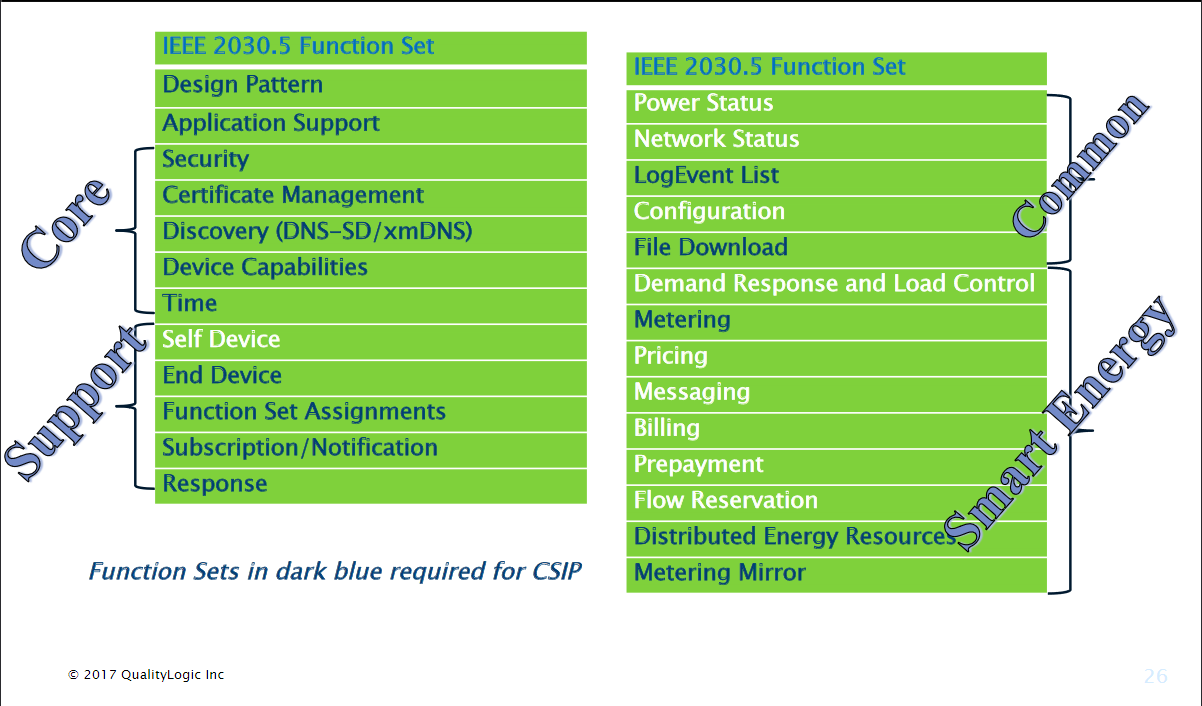
\includegraphics[width=\textwidth]{QualityLogic_FS.png}}
    \end{center}
    \caption{IEEE 2030.5 function sets as grouped by QualityLogic \cite[]{20305workshop}}
\end{figure}

Figure 5.8 shows these groupings, and which of these function sets are required for California SIP.
These groupings provide us with a starting point for determining the priority of function sets, where by those required for California SIP will be implemented first.
An exception to this is the Demand Response and Load Control function set, which has been deemed relevant for DER in Australia by electric utilities in Queensland, and as such it's implementation will be prioritised. \cite[]{QueenslandDER}

Regardless, the groupings in Figure 5.8 further indicate the dependencies between function sets. For example the Device Capabilities function set describes the function sets available on a server, and is therefore used to discover the URI of resources for other function sets.

The conclusion to draw from this is that function sets on the left side of Figure 5.8 are very much depended upon by function sets on the right side, as they describe the core functionality on the client.
Our development will begin on the Security, Certificate Management, and Application Support function sets as part of the common library, where the Application Support function set refers to the use of prescribed technologies, such as TCP, HTTP/1.1 and XML.


\subsection{Testing}
As expected, our client library will be developed alongside a suite of tests. Unlike the common library, these tests will be comprised of both unit and system tests.
System tests will primarily be used to check for conformance to the IEEE 2030.5 specification, using the example system outputs in the specification.
The actual software framework to be used for conducting system tests is yet to be determined, but the requirements to use such a framework are relatively straightforward, obviously requiring both a test client binary, and a mock server.


\subsubsection{Test Client Binary}
In order to perform system tests we will need to wrap our client library in code that can be used to produce a binary that matches a potential use case.
This binary client will be a demonstration of all implemented functionality.
Furthermore, this client binary will act as documentation for device manufacturers using our library.
Producing a test client binary for demonstration was an approach also taken by EPRI in their IEEE 2030.5 client implementation.

\subsubsection{Mock Server}

When it comes to writing system tests, our testing philosophy is hindered by a lack of open-source IEEE 2030.5 implementations, in-development or otherwise.
As such, we'll need to create our own mock IEEE 2030.5 server to test both the sending and receiving of resources from our client.
Neel Bhaskar, as part of UNSW CSE, developed a portion of a working IEEE 2030.5 Server in 2022, and with changes to support hardcoded resources and routes, will be used as the starting point for this mock server.
We will also need to make changes to this server in order for it to use our common library, where we will therefore gain a better idea of what functionality is common to both client \& server.

Specific client functionality, such as the subscription/notification method of resource retrieval, may require extensive work on this mock server. 
As a result, we won't rule out the possibility of writing code that could be reused in a future server implementation.









